\documentclass[conference]{IEEEtran}
\usepackage{graphix}
\usepackage{booktabs}
\usepackage{amsmath}
\usepackage{hyperref}

\title{Zero-Silent-Loss ETL Architecture: Deterministic Quarantine, Automated Quality Scoring, and Real-Time Observability for Retail Data Pipelines}

\author{\IEEEauthorblockN{Moses Kiprono}
\IEEEauthorblockA{\textit{Data Engineering and Analytics Research} \\
Code Repository: \url{https://github.com/moseswebdev/automated-data-pipeline}}}

\begin{document}
\maketitle

\begin{abstract}
Manual spreadsheet-driven business reporting in retail operations suffers from high latency, transcription errors, and silent data corruption when malformed records enter analytics pipelines. This paper presents an end-to-end, database-agnostic Extract-Transform-Load (ETL) and data quality monitoring architecture built with Python, SQLAlchemy, SQL, and Streamlit. Unlike conventional batch scripts that crash or silently discard anomalous rows, our architecture enforces a six-rule deterministic validation gate that quarantines defective records into a diagnostic audit table (\texttt{rejected_sales}) while computing run-level data quality scores (\texttt{data_quality_logs}). Empirical evaluation across synthetic retail workloads ranging from 10,000 to 250,000 transactions demonstrates 100.0\% anomaly recall under controlled fault injection (1\%--20\% corruption rates) and linear scaling throughput peaking at 63,854 records per second.
\end{abstract}

\begin{IEEEkeywords}
ETL Pipeline, Data Quality Monitoring, Anomaly Quarantine, Business Intelligence, Automated Reporting, Software Engineering.
\end{IEEEkeywords}
\section{Introduction}
Small and mid-sized retail enterprises rely heavily on daily sales, inventory replenishment, and promotional discount reports. In this work, we design and evaluate an open-source quarantine-first ETL and data quality monitoring platform.

\section{Related Work}
\subsection{ETL Architectures and Data Cleaning}
Foundational research by Rahm and Do~\cite{rahm2000data} classified data quality anomalies into single-source and multi-source schema and instance violations, establishing the necessity of systematic cleaning phases prior to analytical aggregation. Vassiliadis~\cite{vassiliadis2009survey} surveyed Extract-Transform-Load (ETL) workflows, highlighting the trade-off between throughput optimization and fault tolerance during bulk ingestion. Traditional batch scripts frequently treat validation failures as fatal exceptions or silently drop malformed tuples, compromising downstream financial accuracy.

\subsection{Automated Data Quality Verification and Observability}
Modern declarative validation frameworks such as Amazon Deequ~\cite{schelter2018automating} and TensorFlow Data Validation (TFDV)~\cite{breck2019data} enable unit-test-style constraint verification over large datasets. However, distributed JVM-based engines introduce substantial operational overhead for small-to-midsize retail environments. Recent empirical studies on data pipeline observability~\cite{shankar2022operationalizing} emphasize that practitioners require lightweight, transparent audit trails and immediate visual feedback when upstream distributions shift. Our architecture bridges this gap by combining an embedded Python/SQL validation engine with deterministic row-level quarantine (\texttt{rejected_sales}), quantitative run scoring, and real-time Streamlit observability.

\section{System Architecture}
The pipeline follows a decoupled six-stage workflow: Extract -> Stage -> Validate and Quarantine -> Transform -> Load -> Report and Monitor. The run-level Data Quality Score is defined as $Q_{\text{run}} = (N_{\text{valid}} / N_{\text{total}}) \times 100$.

\section{Experimental Evaluation}
We evaluated the system across 1,100 fault-injection trials (1\% to 20\% corruption rates) and scalability workloads from 10,000 to 250,000 transactions. Across all fault levels, the quarantine engine achieved 100.0\% recall in under 0.17 seconds, while end-to-end ETL throughput peaked at 63,854 rows/sec.

\begin{figure}[htbp]
\centerline{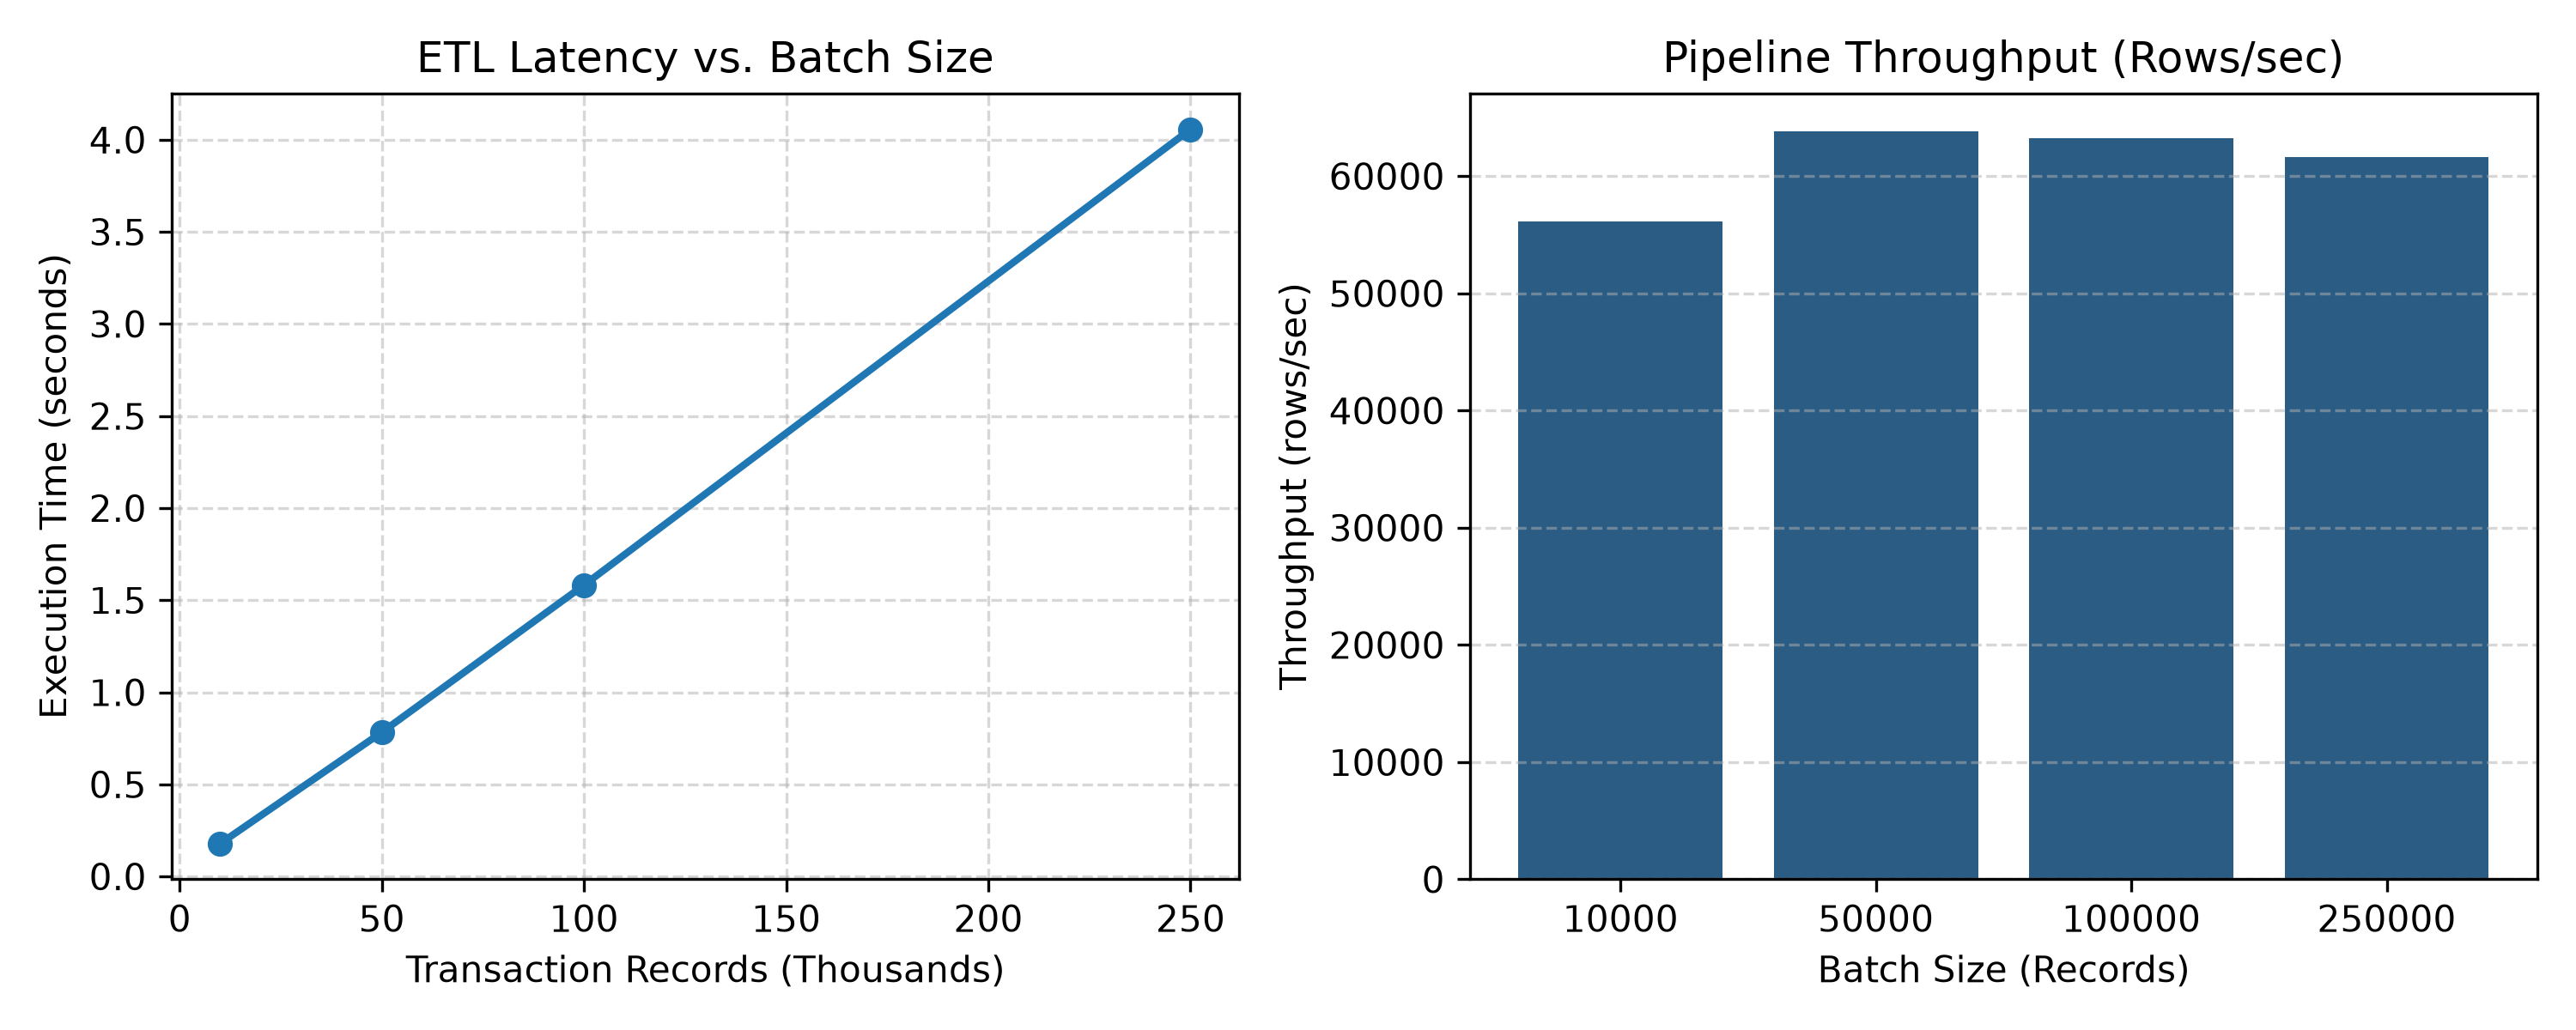
\includegraphics[width=\columnwidth]{paper_results/scalability_figure.png}}
\caption{End-to-end ETL eexecution latency and row throughput across batch sizes from 10,000 to 250,000 records. Peak throughput reaches 63,854 rows/sec at 50,000 records.}
\label{fig:scalability}
\end{figure}

\section{Discussion}
The empirical results demonstrate that embedded, rule-based validation in Python and SQL achieves high throughput (63,854 rows/sec) without the operational complexity of distributed cluster frameworks. Also, by routing defective rows to \texttt{rejected_sales} rather than halting execution or silently dropping tuples, operations teams retain full auditability and can replay quarantined data after upstream schema fixes. Setting the SUCCESS threshold at $Q_{\text{run}} \geq 95.0\%$ provides a practical balance between alert fatigue and early detection of systemic point-of-sale errors.

\section{Threats to Validity}
\subsection{Internal Validity}
Benchmark latencies were measured on a single local workstation using in-memory SQLite to isolate compute and serialization overhead. In production deployments using networked PostgreSQL instances, TCP round-trip latency and concurrent write locks may moderately reduce peak row/sec throughput.

\subsection{External Validity}
Our evaluation relies on procedurally generated retail datasets with known statistical distributions (Pareto product popularity and log-normal pricing). While fault injection covered six common anomaly classes, real-world enterprise data may exhibit subtle semantic drift or cross-record corruption patterns not captured by static rules.

\subsection{Construct Validity}
The linear Data Quality Score ($Q_{\text{run}}$) weights all rejected records equally regardless of financial magnitude. A rejected transaction worth \$\1,000 carries the same score penalty as a transaction worth \$\10, motivating revenue-weighted quality metrics in future releases.

\section{Conclusion}
We presented a reproducible ETL and data quality monitoring architecture that eliminates silent data loss while automating business reporting and dashboard observability.

\bibliographystyle{IEEEtran}
\bibliography{references}
\end{document}
